\section{Parallel KNN}

% See ESLII page 33
% See Dirk page
\begin{itemize}
    \item The $k^{th}$ Nearest-Neighbor (k-NN) methods use observations in the training set $T$ closest in feature space to a given unknown sample $\bm{x}$ to directly find its corresponding prediction $\overline{y}$
    \item The prediction for the k-NN classifier is usually calculated as 
    \[
        \overline{y} \left( \bm{x} \right) = \sum_{\bm{x}_{i} \in N_{k} (\bm{x})} y_{i}
    \]
    \item The notion of 'clostest' implies the use of some sort of meteric. More often than not, feature vectors belong to $\mathbb{R}^{n}$ allowing us to use commonly used metrics to define distance between vectors in our feature space. For our purposes, we shall use the Euclidean norm as a measurement of determining how close two feature values are to each other. The Euclidean norm is simply defined as
    \[
        d \left( \bm{x}, \bm{y} \right) = \left( \sum_{i=1}^{n} \left( x_{i} - y_{i} \right)^{2} \right)^{\frac{1}{2}}
    \]
    \item When a unknown sample $\bm{x}$ is to be classified, a k-NN classifier computes the distance between $\bm{x}$ and the other points within the training set $T$. The training data is then sorted by distance and the $k^{th}$ closests training samples are then used to predict $\bm{x}$.
    \item A simple K-NN algorithm works as follows
\end{itemize}
\begin{algorithm}[ht!]
\caption{Serial k-NN}
\label{alg:serial-k-NN}
\footnotesize
\SetAlgoLined
    \SetKwInOut{Input}{input}\SetKwInOut{Output}{output}
    
    \Input{Training data $T$, an unlabelled sample $\bm{x}$ and a value $k$}
    \Output{Predicted class $\overline{y} \left( \bm{x} \right)$}
    \BlankLine
    Computes distance $d \left( \bm{x}, \bm{x}_{t_i} \right)$ for each $\bm{x}_{t_i} \in T$\;
    $N_{k} (\bm{x}) \gets$ the $k^{th}$ closest $\bm{x}_{t_i}$ determined by $d \left( \bm{x}, \bm{x}_{t_i} \right)$\;
    $\overline{y} \left( \bm{x} \right) \gets \sum_{\bm{x}_{i} \in N_{k} (\bm{x})} y_{i}$\;
    \KwResult{$\overline{y} \left( \bm{x} \right)$}
    \BlankLine
\end{algorithm}
\begin{itemize}
    \item While this method is simple, computing the distance between $\bm{x}$ and each $\bm{x}_{t_i} \in T$ can incur a large time overhead, especially for large training sets
    \item One important observation is that computing the distances $d \left( \bm{x}, \bm{x}_{t_i} \right)$ and $d \left( \bm{x}, \bm{x}_{t_j} \right)$ where $\bm{x}_{t_i}, \bm{x}_{t_j} \in T$ and $i \neq j$ may be done completely independently of each other meaning these computations may be carried out on separate processes.
    \item CITATION takes advantage of this independence to have distance computation carried out on different processes.
\end{itemize}

\begin{algorithm}[ht!]
\caption{Parallel k-NN}
\label{alg:parallel-k-NN}
\footnotesize
\SetAlgoLined
    \SetKwInOut{Input}{input}\SetKwInOut{Output}{output}
    \Input{Training data $T$, an unlabelled sample $\bm{x}$, a value $k$ and the number of processes to perform the algorithm $p$}
    \Output{Predicted class $\overline{y} \left( \bm{x} \right)$}
    \BlankLine
    $\left\lbrace T_{1} , T_{2}, \ldots , T_{p} \right\rbrace \gets$ an equal partition of $T$\;
    \For{$T_{i} \in \left\lbrace T_{1} , T_{2}, \ldots , T_{p} \right\rbrace$ {\bf concurrently}}{
        $N_{k_i} (\bm{x}) \gets$ the $k^{th}$ nearest neighbors from $T_{i}$\;
    }
    $N_{k} (\bm{x}) \gets$ the $k^{th}$ closest neighbors from $N_{k_1} (\bm{x}), N_{k_2} (\bm{x}), \ldots N_{k_p} (\bm{x})$\;
    $\overline{y} \left( \bm{x} \right) \gets \sum_{\bm{x}_{i} \in N_{k} (\bm{x})} y_{i}$\;
    \KwResult{$\overline{y} \left( \bm{x} \right)$}
    \BlankLine
\end{algorithm}
This algorithm is shown pictorially below
\begin{figure}[h]
    \captionsetup[subfigure]{labelformat=empty}
    \centering
    \subfloat[]{
        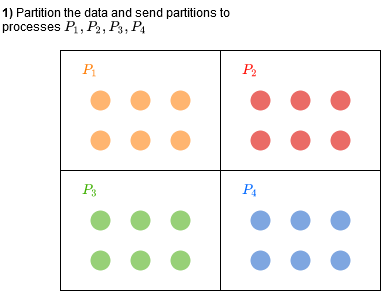
\includegraphics[scale=0.5]{img/STAT4402_tut_KNN_1.png}
    }
    \subfloat[]{
        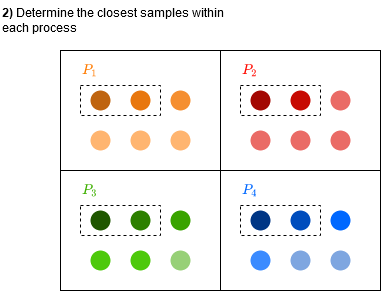
\includegraphics[scale=0.5]{img/STAT4402_tut_KNN_2.png}
    }
    \quad
    \subfloat[]{
        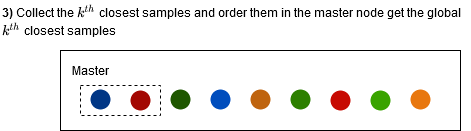
\includegraphics[scale=0.7]{img/STAT4402_tut_KNN_3.png}
    }
    \label{fig:STAT4402_tut_KNN}
\end{figure}